\documentclass[zad,zawodnik,utf8]{sinol}

\title{K-krotne składanie}
\id{kks}
\author{Przemysław Jakub Kozłowski} % Autor zadania
\pagestyle{fancy}
\iomode{stdin}
\konkurs{XIII obóz informatyczny}
\etap{początkująca}
\day{4}
\date{29.09.2016}
\RAM{32}

\begin{document}
\begin{tasktext}%
Przemek zajmuje się informatyką i matematyką. Ostatnio zainteresował się tablicami o rozmiarze $n$, w których występują wszystkie liczby naturalne od $0$ do $n-1$ w dowolnej kolejności (i każda z nich występuje dokładnie raz). Takie tablice czasami nazywane są \textit{permutacjami}.

Przemek musi przekształcać permutacje w swoich obliczeniach matematycznych. Bardzo często musi wykonywać przekształcenie nazywane \textit{złożeniem permutacji}.  To przekształcenie jest bardzo żmudne i wymaga dużo czasu oraz dobrej pamięci (lub dużo miejsca w brudnopisie). Na szczęście Przemek umie również programować, więc napisał program, który będzie za niego wykonywał przekształcenie permutacji. Oto ten program:

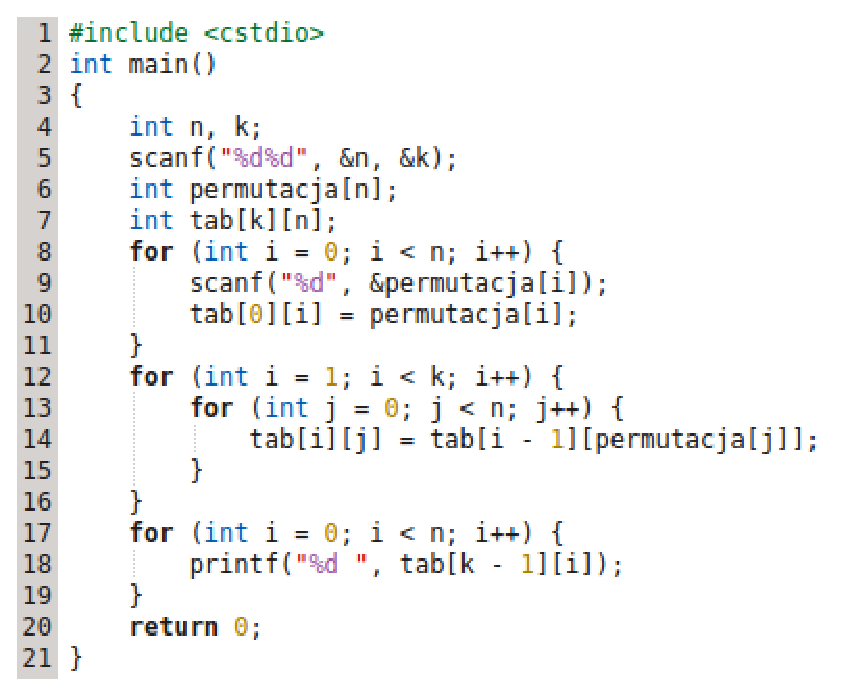
\includegraphics[height=7cm]{Kod.eps}

Niestety po skompilowaniu oraz uruchomieniu okazało się, że program wymaga zbyt dużo pamięci, a czas działania jest zbyt długi. To spowodowało, że Przemek mógł wykonywać przekształcenia jedynie na bardzo małych permutacjach. Możesz się o tym przekonać sam na własnej skórze. Po wysłaniu powyższego algorytmu na sprawdzarkę, dostaniesz jedynie $10$ punktów.

Przemek był bardzo smutny, ale przypomniał sobie o swoim koledze, który jest bardziej doświadczonym programistą. Jesteś nim Ty i Twoim zadaniem jest napisanie własnego algorytmu (lub przerobienie powyższego) tak, aby działał on wystarczająco szybko oraz mieścił się w podanym limicie pamięci dla ograniczeń podanych w sekcji \textit{Wejście}. Jeśli jednak nie potrafisz tego zrobić to możesz wysłać powyższy algorytm na sprawdzarkę.

Jeśli uda Ci się zoptymalizować jedynie pamięć, a czas działania pozostanie taki sam to dostaniesz $50$ punktów.

  \section{Wejście}
W pierwszym wierszu standardowego wejścia znajdują się dwie liczby całkowite $n$ oraz $k$ ($1 \leq k \leq n \leq 10^6$), oznaczające odpowiednio rozmiar permutacji oraz parametr $k$ oznaczający liczbę iteracji pierwszej pętli w algorytmie Przemka. Drugi wiersz przedstawia tablicę, która jest \textit{permutacją} o rozmiarze $n$. Znajduje się w nim $n$ parami różnych liczb naturalnych z przedziału $[0,n-1]$.

  \section{Wyjście}
Pierwszy i jedyny wiersz standardowego wyjścia powinien zawierać $n$ różnych liczb naturalnych z przedziału $[1,n]$. Ten wynik powinien być taki sam jak wynik algorytmu napisanego przez Przemka.

\makecompactexample

\end{tasktext}
\end{document}
